
\documentclass[journal,12pt,twocolumn]{IEEEtran}
%
\usepackage{setspace}
\usepackage{gensymb}
%\doublespacing
\singlespacing

%\usepackage{graphicx}
%\usepackage{amssymb}
%\usepackage{relsize}
\usepackage[cmex10]{amsmath}
%\usepackage{amsthm}
%\interdisplaylinepenalty=2500
%\savesymbol{iint}
%\usepackage{txfonts}
%\restoresymbol{TXF}{iint}
%\usepackage{wasysym}
\usepackage{amsthm}
%\usepackage{iithtlc}
\usepackage{mathrsfs}
\usepackage{txfonts}
\usepackage{stfloats}
\usepackage{bm}
\usepackage{cite}
\usepackage{cases}
\usepackage{subfig}
%\usepackage{xtab}
\usepackage{longtable}
\usepackage{multirow}
%\usepackage{algorithm}
%\usepackage{algpseudocode}
\usepackage{enumitem}
\usepackage{mathtools}
\usepackage{tikz}
\usepackage[american]{circuitikz}
\usepackage{verbatim}
\usepackage{tfrupee}
\usepackage[breaklinks=true]{hyperref}
%\usepackage{stmaryrd}
\usepackage{tkz-euclide} % loads  TikZ and tkz-base
\usetkzobj{all}
\usetikzlibrary{decorations.markings}
\usetikzlibrary{shapes.geometric}
\newif\iflabrev
\usepackage{listings}
    \usepackage{color}                                            %%
    \usepackage{array}                                            %%
    \usepackage{longtable}                                        %%
    \usepackage{calc}                                             %%
    \usepackage{multirow}                                         %%
    \usepackage{hhline}                                           %%
    \usepackage{ifthen}                                           %%
  %optionally (for landscape tables embedded in another document): %%
    \usepackage{lscape}     
\usepackage{multicol}
\usepackage{chngcntr}
%\usepackage{enumerate}

%\usepackage{wasysym}
%\newcounter{MYtempeqncnt}
\DeclareMathOperator*{\Res}{Res}
%\renewcommand{\baselinestretch}{2}
\renewcommand\thesection{\arabic{section}}
\renewcommand\thesubsection{\thesection.\arabic{subsection}}
\renewcommand\thesubsubsection{\thesubsection.\arabic{subsubsection}}

\renewcommand\thesectiondis{\arabic{section}}
\renewcommand\thesubsectiondis{\thesectiondis.\arabic{subsection}}
\renewcommand\thesubsubsectiondis{\thesubsectiondis.\arabic{subsubsection}}

% correct bad hyphenation here
\hyphenation{op-tical net-works semi-conduc-tor}
\def\inputGnumericTable{}                                 %%

\lstset{
%language=C,
frame=single, 
breaklines=true,
columns=fullflexible
}
%\lstset{
%language=tex,
%frame=single, 
%breaklines=true
%}

\begin{document}
%


\newtheorem{theorem}{Theorem}[section]
\newtheorem{problem}{Problem}
\newtheorem{proposition}{Proposition}[section]
\newtheorem{lemma}{Lemma}[section]
\newtheorem{corollary}[theorem]{Corollary}
\newtheorem{example}{Example}[section]
\newtheorem{definition}[problem]{Definition}
%\newtheorem{thm}{Theorem}[section] 
%\newtheorem{defn}[thm]{Definition}
%\newtheorem{algorithm}{Algorithm}[section]
%\newtheorem{cor}{Corollary}
\newcommand{\BEQA}{\begin{eqnarray}}
\newcommand{\EEQA}{\end{eqnarray}}
\newcommand{\define}{\stackrel{\triangle}{=}}
\bibliographystyle{IEEEtran}
%\bibliographystyle{ieeetr}
\providecommand{\mbf}{\mathbf}
\providecommand{\pr}[1]{\ensuremath{\Pr\left(#1\right)}}
\providecommand{\qfunc}[1]{\ensuremath{Q\left(#1\right)}}
\providecommand{\sbrak}[1]{\ensuremath{{}\left[#1\right]}}
\providecommand{\lsbrak}[1]{\ensuremath{{}\left[#1\right.}}
\providecommand{\rsbrak}[1]{\ensuremath{{}\left.#1\right]}}
\providecommand{\brak}[1]{\ensuremath{\left(#1\right)}}
\providecommand{\lbrak}[1]{\ensuremath{\left(#1\right.}}
\providecommand{\rbrak}[1]{\ensuremath{\left.#1\right)}}
\providecommand{\cbrak}[1]{\ensuremath{\left\{#1\right\}}}
\providecommand{\lcbrak}[1]{\ensuremath{\left\{#1\right.}}
\providecommand{\rcbrak}[1]{\ensuremath{\left.#1\right\}}}
\theoremstyle{remark}
\newtheorem{rem}{Remark}
\newcommand{\sgn}{\mathop{\mathrm{sgn}}}
\providecommand{\abs}[1]{\left\vert#1\right\vert}
\providecommand{\res}[1]{\Res\displaylimits_{#1}} 
\providecommand{\norm}[1]{\left\lVert#1\right\rVert}
%\providecommand{\norm}[1]{\lVert#1\rVert}
\providecommand{\mtx}[1]{\mathbf{#1}}
\providecommand{\mean}[1]{E\left[ #1 \right]}
\providecommand{\fourier}{\overset{\mathcal{F}}{ \rightleftharpoons}}
%\providecommand{\hilbert}{\overset{\mathcal{H}}{ \rightleftharpoons}}
\providecommand{\system}{\overset{\mathcal{H}}{ \longleftrightarrow}}
	%\newcommand{\solution}[2]{\textbf{Solution:}{#1}}
\newcommand{\solution}{\noindent \textbf{Solution: }}
\newcommand{\cosec}{\,\text{cosec}\,}
\providecommand{\dec}[2]{\ensuremath{\overset{#1}{\underset{#2}{\gtrless}}}}
\newcommand{\myvec}[1]{\ensuremath{\begin{pmatrix}#1\end{pmatrix}}}
\newcommand{\mydet}[1]{\ensuremath{\begin{vmatrix}#1\end{vmatrix}}}
%\numberwithin{equation}{section}
\numberwithin{equation}{subsection}
%\numberwithin{problem}{section}
%\numberwithin{definition}{section}
\makeatletter
\@addtoreset{figure}{problem}
\makeatother
\let\StandardTheFigure\thefigure
\let\vec\mathbf
%\renewcommand{\thefigure}{\theproblem.\arabic{figure}}
\renewcommand{\thefigure}{\theproblem}
%\setlist[enumerate,1]{before=\renewcommand\theequation{\theenumi.\arabic{equation}}
%\counterwithin{equation}{enumi}
%\renewcommand{\theequation}{\arabic{subsection}.\arabic{equation}}
\def\putbox#1#2#3{\makebox[0in][l]{\makebox[#1][l]{}\raisebox{\baselineskip}[0in][0in]{\raisebox{#2}[0in][0in]{#3}}}}
     \def\rightbox#1{\makebox[0in][r]{#1}}
     \def\centbox#1{\makebox[0in]{#1}}
     \def\topbox#1{\raisebox{-\baselineskip}[0in][0in]{#1}}
     \def\midbox#1{\raisebox{-0.5\baselineskip}[0in][0in]{#1}}
\vspace{3cm}
\title{
%	\logo{
Control Systems
%	}
}
\author{ G V V Sharma$^{*}$% <-this % stops a space
	\thanks{*The author is with the Department
		of Electrical Engineering, Indian Institute of Technology, Hyderabad
		502285 India e-mail:  gadepall@iith.ac.in. All content in this manual is released under GNU GPL.  Free and open source.}
	
}	
%\title{
%	\logo{Matrix Analysis through Octave}{\begin{center}\includegraphics[scale=.24]{tlc}\end{center}}{}{HAMDSP}
%}
% paper title
% can use linebreaks \\ within to get better formatting as desired
%\title{Matrix Analysis through Octave}
%
%
% author names and IEEE memberships
% note positions of commas and nonbreaking spaces ( ~ ) LaTeX will not break
% a structure at a ~ so this keeps an author's name from being broken across
% two lines.
% use \thanks{} to gain access to the first footnote area
% a separate \thanks must be used for each paragraph as LaTeX2e's \thanks
% was not built to handle multiple paragraphs
%
%\author{<-this % stops a space
%\thanks{}}
%}
% note the % following the last \IEEEmembership and also \thanks - 
% these prevent an unwanted space from occurring between the last author name
% and the end of the author line. i.e., if you had this:
% 
% \author{....lastname \thanks{...} \thanks{...} }
%                     ^------------^------------^----Do not want these spaces!
%
% a space would be appended to the last name and could cause every name on that
% line to be shifted left slightly. This is one of those "LaTeX things". For
% instance, "\textbf{A} \textbf{B}" will typeset as "A B" not "AB". To get
% "AB" then you have to do: "\textbf{A}\textbf{B}"
% \thanks is no different in this regard, so shield the last } of each \thanks
% that ends a line with a % and do not let a space in before the next \thanks.
% Spaces after \IEEEmembership other than the last one are OK (and needed) as
% you are supposed to have spaces between the names. For what it is worth,
% this is a minor point as most people would not even notice if the said evil
% space somehow managed to creep in.
% The paper headers
%\markboth{Journal of \LaTeX\ Class Files,~Vol.~6, No.~1, January~2007}%
%{Shell \MakeLowercase{\textit{et al.}}: Bare Demo of IEEEtran.cls for Journals}
% The only time the second header will appear is for the odd numbered pages
% after the title page when using the twoside option.
% 
% *** Note that you probably will NOT want to include the author's ***
% *** name in the headers of peer review papers.                   ***
% You can use \ifCLASSOPTIONpeerreview for conditional compilation here if
% you desire.
% If you want to put a publisher's ID mark on the page you can do it like
% this:
%\IEEEpubid{0000--0000/00\$00.00~\copyright~2007 IEEE}
% Remember, if you use this you must call \IEEEpubidadjcol in the second
% column for its text to clear the IEEEpubid mark.
% make the title area
\maketitle
\newpage
\tableofcontents
\bigskip
\renewcommand{\thefigure}{\theenumi}
\renewcommand{\thetable}{\theenumi}
%\renewcommand{\theequation}{\theenumi}
%\begin{abstract}
%%\boldmath
%In this letter, an algorithm for evaluating the exact analytical bit error rate  (BER)  for the piecewise linear (PL) combiner for  multiple relays is presented. Previous results were available only for upto three relays. The algorithm is unique in the sense that  the actual mathematical expressions, that are prohibitively large, need not be explicitly obtained. The diversity gain due to multiple relays is shown through plots of the analytical BER, well supported by simulations. 
%
%\end{abstract}
% IEEEtran.cls defaults to using nonbold math in the Abstract.
% This preserves the distinction between vectors and scalars. However,
% if the journal you are submitting to favors bold math in the abstract,
% then you can use LaTeX's standard command \boldmath at the very start
% of the abstract to achieve this. Many IEEE journals frown on math
% in the abstract anyway.
% Note that keywords are not normally used for peerreview papers.
%\begin{IEEEkeywords}
%Cooperative diversity, decode and forward, piecewise linear
%\end{IEEEkeywords}
% For peer review papers, you can put extra information on the cover
% page as needed:
% \ifCLASSOPTIONpeerreview
% \begin{center} \bfseries EDICS Category: 3-BBND \end{center}
% \fi
%
% For peerreview papers, this IEEEtran command inserts a page break and
% creates the second title. It will be ignored for other modes.
%\IEEEpeerreviewmaketitle

\begin{abstract}
This manual is an introduction to control systems based on GATE problems.Links to sample Python codes are available in the text.  
\end{abstract}
Download python codes using 
\begin{lstlisting}
svn co https://github.com/gadepall/school/trunk/control/codes
\end{lstlisting}
\section{Feedback Circuits}
\begin{enumerate}[label=\thesubsection.\arabic*.,ref=\thesubsection.\theenumi]
\numberwithin{equation}{enumi}

\item
A dc amplifier has an open loop gain of 1000 and two poles, a dominant one at 1kHz and a high frequency one whose location can be controlled. It is required to connect this amplifier in a negative feedback loop that provides a dc closed loop gain of 10 and a maximally flat response.Find the required value of H.
\\
\solution Given, open loop gain G is dependent on frequency and has two poles.Therefore,G(s) can be written as..,
\begin{align}
  G(s) &= \frac{G_0}{(1-\frac{s}{p_{1}})(1-\frac{s}{p_{2}})} \label{eq:open_loop_gain} 
\end{align}
where, p1 and p2 are poles of G(s).
Parameters given are shown in Table.\ref{table:Input_Table}:1
\begin{table}[!ht]
\centering

%%%%%%%%%%%%%%%%%%%%%%%%%%%%%%%%%%%%%%%%%%%%%%%%%%%%%%%%%%%%%%%%%%%%%%
%%                                                                  %%
%%  This is the header of a LaTeX2e file exported from Gnumeric.    %%
%%                                                                  %%
%%  This file can be compiled as it stands or included in another   %%
%%  LaTeX document. The table is based on the longtable package so  %%
%%  the longtable options (headers, footers...) can be set in the   %%
%%  preamble section below (see PRAMBLE).                           %%
%%                                                                  %%
%%  To include the file in another, the following two lines must be %%
%%  in the including file:                                          %%
%%        \def\inputGnumericTable{}                                 %%
%%  at the beginning of the file and:                               %%
%%        \input{name-of-this-file.tex}                             %%
%%  where the table is to be placed. Note also that the including   %%
%%  file must use the following packages for the table to be        %%
%%  rendered correctly:                                             %%
%%    \usepackage[latin1]{inputenc}                                 %%
%%    \usepackage{color}                                            %%
%%    \usepackage{array}                                            %%
%%    \usepackage{longtable}                                        %%
%%    \usepackage{calc}                                             %%
%%    \usepackage{multirow}                                         %%
%%    \usepackage{hhline}                                           %%
%%    \usepackage{ifthen}                                           %%
%%  optionally (for landscape tables embedded in another document): %%
%%    \usepackage{lscape}                                           %%
%%                                                                  %%
%%%%%%%%%%%%%%%%%%%%%%%%%%%%%%%%%%%%%%%%%%%%%%%%%%%%%%%%%%%%%%%%%%%%%%



%%  This section checks if we are begin input into another file or  %%
%%  the file will be compiled alone. First use a macro taken from   %%
%%  the TeXbook ex 7.7 (suggestion of Han-Wen Nienhuys).            %%
\def\ifundefined#1{\expandafter\ifx\csname#1\endcsname\relax}


%%  Check for the \def token for inputed files. If it is not        %%
%%  defined, the file will be processed as a standalone and the     %%
%%  preamble will be used.                                          %%
\ifundefined{inputGnumericTable}

%%  We must be able to close or not the document at the end.        %%
	\def\gnumericTableEnd{\end{document}}


%%%%%%%%%%%%%%%%%%%%%%%%%%%%%%%%%%%%%%%%%%%%%%%%%%%%%%%%%%%%%%%%%%%%%%
%%                                                                  %%
%%  This is the PREAMBLE. Change these values to get the right      %%
%%  paper size and other niceties.                                  %%
%%                                                                  %%
%%%%%%%%%%%%%%%%%%%%%%%%%%%%%%%%%%%%%%%%%%%%%%%%%%%%%%%%%%%%%%%%%%%%%%

	\documentclass[12pt%
			  %,landscape%
                    ]{report}
       \usepackage[latin1]{inputenc}
       \usepackage{fullpage}
       \usepackage{color}
       \usepackage{array}
       \usepackage{longtable}
       \usepackage{calc}
       \usepackage{multirow}
       \usepackage{hhline}
       \usepackage{ifthen}



%%  End of the preamble for the standalone. The next section is for %%
%%  documents which are included into other LaTeX2e files.          %%
\else

%%  We are not a stand alone document. For a regular table, we will %%
%%  have no preamble and only define the closing to mean nothing.   %%
    \def\gnumericTableEnd{}

%%  If we want landscape mode in an embedded document, comment out  %%
%%  the line above and uncomment the two below. The table will      %%
%%  begin on a new page and run in landscape mode.                  %%
%       \def\gnumericTableEnd{\end{landscape}}
%       \begin{landscape}


%%  End of the else clause for this file being \input.              %%
\fi

%%%%%%%%%%%%%%%%%%%%%%%%%%%%%%%%%%%%%%%%%%%%%%%%%%%%%%%%%%%%%%%%%%%%%%
%%                                                                  %%
%%  The rest is the gnumeric table, except for the closing          %%
%%  statement. Changes below will alter the table's appearance.     %%
%%                                                                  %%
%%%%%%%%%%%%%%%%%%%%%%%%%%%%%%%%%%%%%%%%%%%%%%%%%%%%%%%%%%%%%%%%%%%%%%

\providecommand{\gnumericmathit}[1]{#1} 
%%  Uncomment the next line if you would like your numbers to be in %%
%%  italics if they are italizised in the gnumeric table.           %%
%\renewcommand{\gnumericmathit}[1]{\mathit{#1}}
\providecommand{\gnumericPB}[1]%
{\let\gnumericTemp=\\#1\let\\=\gnumericTemp\hspace{0pt}}
 \ifundefined{gnumericTableWidthDefined}
        \newlength{\gnumericTableWidth}
        \newlength{\gnumericTableWidthComplete}
        \newlength{\gnumericMultiRowLength}
        \global\def\gnumericTableWidthDefined{}
 \fi
%% The following setting protects this code from babel shorthands.  %%
 \ifthenelse{\isundefined{\languageshorthands}}{}{\languageshorthands{english}}
%%  The default table format retains the relative column widths of  %%
%%  gnumeric. They can easily be changed to c, r or l. In that case %%
%%  you may want to comment out the next line and uncomment the one %%
%%  thereafter                                                      %%
\providecommand\gnumbox{\makebox[0pt]}
%%\providecommand\gnumbox[1][]{\makebox}

%% to adjust positions in multirow situations                       %%
\setlength{\bigstrutjot}{\jot}
\setlength{\extrarowheight}{\doublerulesep}

%%  The \setlongtables command keeps column widths the same across  %%
%%  pages. Simply comment out next line for varying column widths.  %%
\setlongtables

\setlength\gnumericTableWidth{%
	53pt+%
	93pt+%
0pt}
\def\gumericNumCols{2}
\setlength\gnumericTableWidthComplete{\gnumericTableWidth+%
         \tabcolsep*\gumericNumCols*2+\arrayrulewidth*\gumericNumCols}
\ifthenelse{\lengthtest{\gnumericTableWidthComplete > \linewidth}}%
         {\def\gnumericScale{\ratio{\linewidth-%
                        \tabcolsep*\gumericNumCols*2-%
                        \arrayrulewidth*\gumericNumCols}%
{\gnumericTableWidth}}}%
{\def\gnumericScale{1}}

%%%%%%%%%%%%%%%%%%%%%%%%%%%%%%%%%%%%%%%%%%%%%%%%%%%%%%%%%%%%%%%%%%%%%%
%%                                                                  %%
%% The following are the widths of the various columns. We are      %%
%% defining them here because then they are easier to change.       %%
%% Depending on the cell formats we may use them more than once.    %%
%%                                                                  %%
%%%%%%%%%%%%%%%%%%%%%%%%%%%%%%%%%%%%%%%%%%%%%%%%%%%%%%%%%%%%%%%%%%%%%%

\ifthenelse{\isundefined{\gnumericColA}}{\newlength{\gnumericColA}}{}\settowidth{\gnumericColA}{\begin{tabular}{@{}p{110pt*\gnumericScale}@{}}x\end{tabular}}
\ifthenelse{\isundefined{\gnumericColB}}{\newlength{\gnumericColB}}{}\settowidth{\gnumericColB}{\begin{tabular}{@{}p{30pt*\gnumericScale}@{}}x\end{tabular}}

\begin{tabular}[c]{%
	b{\gnumericColA}%
	b{\gnumericColB}%
	}

%%%%%%%%%%%%%%%%%%%%%%%%%%%%%%%%%%%%%%%%%%%%%%%%%%%%%%%%%%%%%%%%%%%%%%
%%  The longtable options. (Caption, headers... see Goosens, p.124) %%
%	\caption{The Table Caption.}             \\	%
% \hline	% Across the top of the table.
%%  The rest of these options are table rows which are placed on    %%
%%  the first, last or every page. Use \multicolumn if you want.    %%

%%  Header for the first page.                                      %%
%	\multicolumn{2}{c}{The First Header} \\ \hline 
%	\multicolumn{1}{c}{colTag}	%Column 1
%	&\multicolumn{1}{c}{colTag}	\\ \hline %Last column
%	\endfirsthead

%%  The running header definition.                                  %%
%	\hline
%	\multicolumn{2}{l}{\ldots\small\slshape continued} \\ \hline
%	\multicolumn{1}{c}{colTag}	%Column 1
%	&\multicolumn{1}{c}{colTag}	\\ \hline %Last column
%	\endhead

%%  The running footer definition.                                  %%
%	\hline
%	\multicolumn{2}{r}{\small\slshape continued\ldots} \\
%	\endfoot

%%  The ending footer definition.                                   %%
%	\multicolumn{2}{c}{That's all folks} \\ \hline 
%	\endlastfoot
%%%%%%%%%%%%%%%%%%%%%%%%%%%%%%%%%%%%%%%%%%%%%%%%%%%%%%%%%%%%%%%%%%%%%%

\hhline{|-|-}
	 \multicolumn{1}{|p{\gnumericColA}|}%
	{\gnumericPB{\centering}\gnumbox{\textbf{Parameter}}}
	&\multicolumn{1}{p{\gnumericColB}|}%
	{\gnumericPB{\centering}\gnumbox{\textbf{Value}}}
\\
\hhline{|-|-}
	 \multicolumn{1}{|p{\gnumericColA}|}%
	{\gnumericPB{\centering}\gnumbox{\text{dc open loop gain}}}
	&\multicolumn{1}{p{\gnumericColB}|}%
	{\gnumericPB{\centering}\gnumbox{\text{1000}}}
\\
\hhline{|-|-}
	 \multicolumn{1}{|p{\gnumericColA}|}%
	{\gnumericPB{\centering}\gnumbox{\text{dominant pole}}}
	&\multicolumn{1}{p{\gnumericColB}|}%
	{\gnumericPB{\centering}\gnumbox{\text{1000Hz}}}
\\
\hhline{|-|-}
	 \multicolumn{1}{|p{\gnumericColA}|}%
	{\gnumericPB{\centering}\gnumbox{\text{insignificant pole}}}
	&\multicolumn{1}{p{\gnumericColB}|}%
	{\gnumericPB{\centering}\gnumbox{\text{$-p_2$}}}
\\
\hhline{|-|-}
	 \multicolumn{1}{|p{\gnumericColA}|}%
	{\gnumericPB{\centering}\gnumbox{\text{dc closed loop gain}}}
	&\multicolumn{1}{p{\gnumericColB}|}%
	{\gnumericPB{\centering}\gnumbox{\text{10}}}
\\

\hhline{|-|-|}
\end{tabular}

\ifthenelse{\isundefined{\languageshorthands}}{}{\languageshorthands{\languagename}}
\gnumericTableEnd

\caption{1}
\label{table:Input_Table}
\end{table}
\begin{align}
    G_0 &= 1000\\
\text{Therefore.,} G(s)&= \frac{1000}{(1-\frac{s}{p_{1}})(1-\frac{s}{p_{2}})}  
\end{align}
Let, p1 be the dominant pole.
\begin{align}
    p_1 &= 2\pi10^3 rad/sec
\end{align}
Now, we connect the system in a negative feedback of feedback factor H.
We know that the closed loop gain of a negative feedback system is.,
\begin{align}
    T(s) &= \frac{G(s)}{1+G(s)H} \label{eq:transfer_function}
\end{align}
But,also given DC closed loop gain is 10. DC closed loop gain is given in equation.\ref{eq:dc_gain} 
\begin{align}
T(0) &= \frac{G_0}{1+G_0H} \label{eq:dc_gain} \\
\text{given.,}T(0)&=10\\
\text{and.,}G_0 &= 1000\\
\frac{1000}{1+1000H} &= 10\\
1+1000H &= 100\\
\implies H &= \frac{99}{1000} = 0.099 \label{eq:h_value}
\end{align}
from equation:\ref{eq:h_value}, the value of H is 0.099.Therefore, the feedback factor is 0.099.
%------------------------------
\item Find the location at which second ple can be placed.\\
\solution Given the negative feedback system should have maximally flat response.from equation.\ref{eq:transfer_function} and equation.\ref{eq:open_loop_gain} the transfer function is,
\begin{align}
    T(s) &= \frac{\frac{G_0}{(1-\frac{s}{p_{1}})(1-\frac{s}{p_{2}})}}{1+\frac{HG_0}{(1-\frac{s}{p_{1}})(1-\frac{s}{p_{2}})}}\\
    T(s) &= \frac{\frac{p_1p_2G_0}{(p_1-s)(p_2-s)}}{1+\frac{p_1p_2HG_0}{(p_1-s)(p_2-s)}}
\end{align}
\begin{align}
    T(s) &= \frac{p_1p_2G_0}{(p_1-s)(p_2-s) + p_1p_2HG_0}\\
    T(s) &= \frac{p_1p_2G_0}{p_1p_2-(p_1+p_2)s+s^2 + p_1p_2HG_0}\\
    T(s) &= \frac{p_1p_2G_0}{s^2-(p_1+p_2)s+(HG_0+1)p_1p_2} \label{eq:closed_loop}
\end{align}
The characteristics equation of above transfer function is.,
\begin{align}
    C.E &= s^2-(p_1+p_2)s+(HG_0+1)p_1p_2 \label{eq:ce}
\end{align}
In general, For a second order amplifier the C.E is.,
\begin{align}
    C.E &= s^2+2\zeta\omega_ns+\omega_n^{2} \label{eq:second_order_ce}
\end{align}
The quality factor Q of equation.\ref{eq:second_order_ce}, is given by
\begin{align}
    Q &= \frac{1}{2\zeta}
\end{align}
From equation.\ref{eq:ce},
\begin{align}
    \omega_n &= \pm{\sqrt{(HG_0+1)p_1p_2}}\\
    \zeta &= \pm{\frac{2p_1p_2}{\sqrt{(HG_0+1)p_1p_2}}}
\end{align}
Therefore,For the given second order amplifier with characteristic equation.\ref{eq:ce},the Q factor is,
\begin{align}
    Q &= \pm{\frac{\sqrt{(1+HG_0)p_1p_2}}{p_1+p_2}} \label{eq:Q}
\end{align}
For a negative feedback amplifier to achieve maximally flat response,
\begin{align}
    Q &= 0.7071\\
\end{align}
Therefore, substituting the values of Q and other parameters in equation.\ref{eq:Q},
\begin{align}
    0.7071 &= \pm{\frac{\sqrt{(1+0.099(1000))(2\pi10^3)p_2}}{2\pi10^3+p_2}}
\end{align}
Squaring on both sides and rearranging.,
\begin{align}
    (1+1000(0.099))2\pi10^3p_2 &= 0.7071^2{(2\pi10^3+p_2)}^2
\end{align}
\begin{align}
    (100)2\pi10^3 = 0.7071^2(2\pi10^3+p_2)^2\\
    \implies 0.5p_2^2-622037.2p_2+19733247.6=0
\end{align}
Solving above equation.,
\begin{align}
p_2 &= 31.7244 \text{ rad/sec}\\
p_2 &= 1244042.676 \text{ rad/sec}
\end{align}
But, Since p1 is dominating pole,p1 should be close to origin.
\begin{align}
    p_1 <<< p_2
\end{align}
\begin{align}
p_2 &= 1.244\text{ Mrad/sec}\\
\\
p_2 &= \frac{1.244M}{2\pi} \text{Hz}= 192.989\text{ kHz}\\
\end{align}
%---------------------
\item Verify roots of above equation using python code.
\begin{lstlisting}
codes/ee18btech11005/ee18btech11005_1.py
\end{lstlisting}
%-----------------
\item Now, Find the open loop transfer function and closed loop transfer function of the system.
\solution Substituting the value of p2 in  the equation \ref{eq:open_loop_gain} and \ref{eq:closed_loop}
\begin{align}
     G(s) &= \frac{1000}{(1-\frac{s}{10^3})(1-\frac{s}{192.989x10^3})}
\end{align}
\begin{align}
    T(s) &= \frac{192.989x10^9}{s^2-193x10^3s+192.989x10^{10}}
\end{align}
%--------------------------
\item Verify from the Bode plot of above closed loop transfer function that it has maximally flat response.\\
\solution The following code generates the bode plot of the transfer function.
\begin{lstlisting}
codes/ee18btech11005/ee18btech11005_2.py
\end{lstlisting}
\begin{figure}[!ht]
\centering
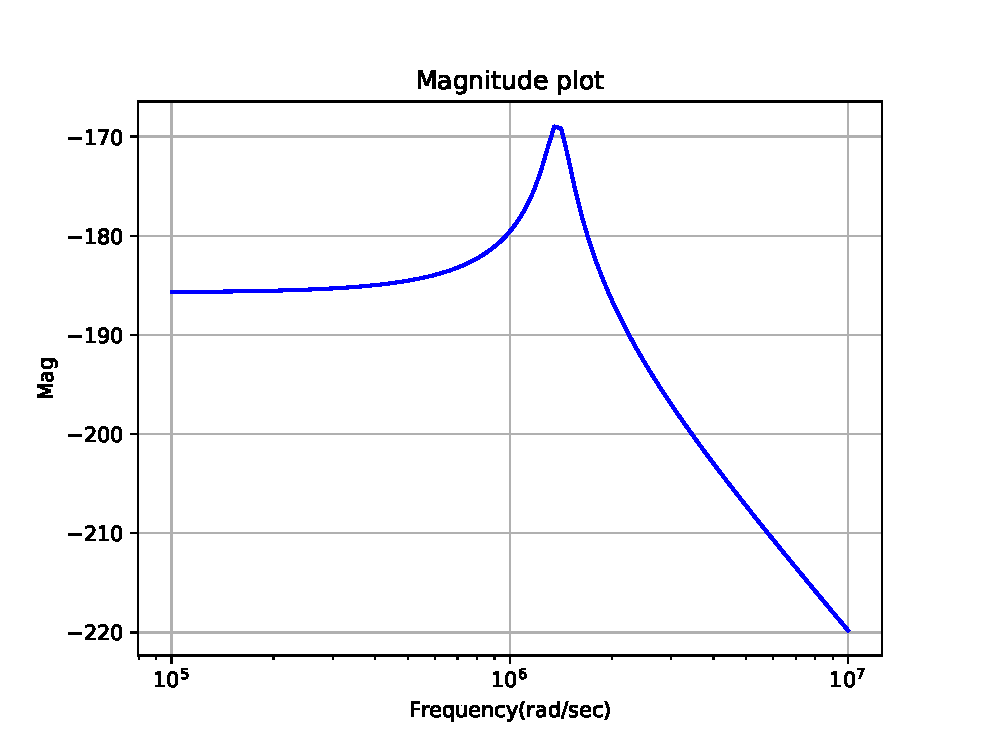
\includegraphics[width=\columnwidth]{./figs/ee18btech11005/ee18btech11005_1.eps}
\caption{1}
\label{fig:ee18btech11005_1}
\end{figure}
From the magnitude bode plot in figure.\ref{fig:ee18btech11005_1}:1 we can tell that the open loop transfer function after having negative feedback has maximally flat response for the obtained value of p2. 
\item Design a circuit that represents the above transfer function.\\
\solution The circuit can be designed using an operational amplifier having negative feedback.Consider the circuit shown in figure.\ref{fig:equivalent_control_system}
\begin{figure}[!ht]
	\begin{center}
			\resizebox{\columnwidth}{!}{
\tikzstyle{block} = [draw, fill=blue!20, rectangle, 
    minimum height=3em, minimum width=4em]
\tikzstyle{sum} = [draw, fill=blue!20, circle, node distance=1cm]
\tikzstyle{input} = [coordinate]
\tikzstyle{output} = [coordinate]
\tikzstyle{pinstyle} = [pin edge={to-,thin,black}]

\begin{tikzpicture}[auto, node distance=2cm]
    \node [input, name=input] {$V_s$};
    \node [sum, right of=input] (sum) {};
    \node [block, right of=sum] (controller) {$G(s)$};
    \node [output, right of=controller] (output) {};
    \node [block, below of=controller] (feedback) {$H = 0.099$};
    \draw [draw,->] (input) -- node {$V_s$} (sum);
    \draw [->] (sum) -- node {$V_i$} (controller);
    \draw [->] (controller) -- node [name=y] {$V_o$}(output);
    \draw [->] (y) |- (feedback);
    \draw [->] (feedback) -| node[pos=0.99]{$-$}  node [near end] {$V_f$} (sum);
\end{tikzpicture}
}
	\end{center}
\caption{}
\label{fig:equivalent_control_system}
\end{figure}
For a differential amplifier,
\begin{align}
  V_o &= G(s)(V_{in} - V) \\
  \text{where.,} V &= \frac{V_oR}{kR}=\frac{V_o}{k}\\
  V_o &= G(s)(V_{in} - \frac{V_o}{k})\\
  V_o &= G(s)V_{in} - \frac{G(s)V_o}{k}\\
  V_o &= \frac{G(s)V_{in}}{1+\frac{G(s)}{k}}
  \end{align}
  \begin{align}
  T(s) &= \frac{G(s)}{1+\frac{G(s)}{k}}\label{eq:Opamp_equivalent}
\end{align}
Where.., G(s) is open loop gain that varies with frequency.
Comparing equation.\ref{eq:transfer_function} and equation.\ref{eq:Opamp_equivalent}
We can design the equivalent circuit for the given problem.
\begin{align}
H &= \frac{1}{k}\\
\implies k &= \frac{1}{H}\\
\end{align}
We know.,H = 0.099
\begin{align}
k &= \frac{1}{0.099} = \frac{1000}{99}\\
k &= 10.101
\end{align}
Choose..,
\begin{align}
    R = 1000 \Omega
\end{align}
So, the final circuit is shown in figure.\ref{fig:final_circuit}.
\begin{figure}[!ht]
	\begin{center}
			\resizebox{\columnwidth}{!}{ \begin{circuitikz}
\ctikzset{bipoles/length=1cm}

\draw 
(0, 0) node[op amp] (opamp) {}
(opamp.-) -- (-1,0.35) -- (-1, 2)--(1.5,2) to[R=$9101\Omega$,*-*] (1.5,0){}
(opamp.out)--(1.5,0){}
(opamp.+) -- (-2,-0.35) node at(-2,-0.5) {$V_{in}$}
(1.5,2) to[R=$1000\Omega$] (1.5,4)--(2,4) node[ground]{}
(1.5,0) -- (2,0)
node at(2,-0.3){$V_o$}
node at(1.7,2){V}
(opamp.center) node[]{{$G(s)$}}
;\end{circuitikz}
}
	\end{center}
\caption{}
\label{fig:final_circuit}
\end{figure}
The above circuit ensures the closed loop transfer function has maximally flat response.
\end{enumerate}


\end{document}
